\documentclass{article}
    \usepackage{amssymb}
    \usepackage{color}
    \usepackage{listings}
    \usepackage{graphicx}
    \usepackage{subcaption}
    \usepackage{geometry}
    \usepackage{float}
    \geometry{
    a4paper,
    total={170mm,257mm},
    left=20mm,
    top=20mm,
    }

    \setlength{\parindent}{0em}
    \setlength{\parskip}{1em} % length of the spacing
    
    \lstset{ % General setup for the package
        language=Python,
        basicstyle=\small\sffamily,
        numbers=left,
        numberstyle=\tiny,
        frame=tb,
        tabsize=4,
        columns=fixed,
        showstringspaces=false,
        showtabs=false,
        keepspaces,
        commentstyle=\color{red},
        keywordstyle=\color{blue},
        emphstyle=\ttb\color{deepred},    
        stringstyle=\color{deepgreen}
    }
    
    \begin{document}
        \begin{figure}
            \centering
            
\includegraphics[width=0.5\linewidth]{./img/vub.png}
        \end{figure}
        \title{Modeling Languages Project Report}
        \author{Juan Jose Soriano Escobar }
        \maketitle
        \newpage

        \tableofcontents
        \newpage
    
        \begin{appendix}
            \listoffigures
          \end{appendix}
          \newpage
    
    
            \section{Introduction}

            Modeling is an important part of any System or product development that helps to understand the model system from a holistic point of view, ensuring that all the functionalities and
            stakeholders requirements are covered. One of the most popular modeling tools nowadays in the software and product development environment is UML.

            UML is a communication standard for the world of software development.  It consists of different types of diagrams that  help to describe the boundary, the structure 
            and the behavior of the system.

            In this report, a Hospital appointment and billing system management are described and modeled in UML as result of the concepts and diagrams learn in the course of Modeling Languages.

            The description of the model in this report will be split by diagram types, covering use case, sequence, activity, state and class diagram.
             
            \newpage         
            \section{Use Case Diagram}

            A use case diagram captures and explains to the stakeholders of a system about its behavior describes the
            system’s behavior under various conditions as it responds to a request from the “primary actor”
            \cite{sysml}.

            The case diagram is also good to ensure that every member in the development team understand the main activities and behavior of the system,
            recognizing the actors and the global interactions among them.

            The use case diagram is divided in three main behaviors, the appointment management, clinical history management and payments.

            \subsection{Appointment Use Case}

            In the figure \ref{fig:Appointment} the use case diagram for the appointment system is Illustrated. It contains four Actors, three Human actors such as the Patient, the Receptionist and the Doctor. 
            The remaining actor is the Hospital System which is consider as a Software from the hospital that is used to manage all the logistics, billing and service operations by different users.

            \begin{figure}[H]
                \centering 
                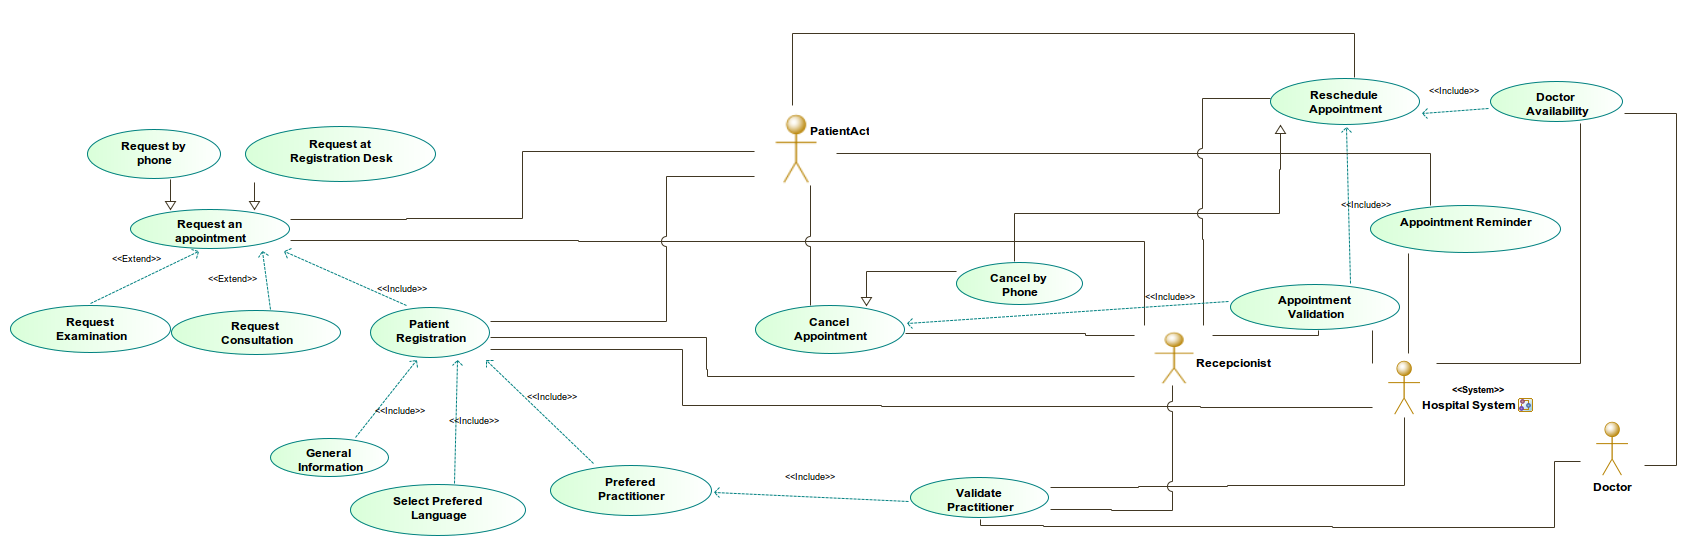
\includegraphics[width=1\linewidth]{./img/appointments.png}
                \setcaptioncitation{Created with Modelio 3.7.}
                \caption{Appoint Use Case Diagram}
                \label{fig:Appointment}
            \end{figure}


            This diagram presents how the patient communicates with the receptionist by phone or at the Hospital desk, to Schedule, cancel or modify an appointment. To do so, the Receptionist has to use the
            system, registering the patient and validating if the doctor is available for the required appointment.

            \subsection{Examination Use Case}

            Once the patient has an appointment scheduled, the next step is to understand the appointment behavior. As actors, there are the same four included in the previous Use Case Diagram plus the appointment considered as a 
            secondary one.

            The day of the appointment, the Patient will go to the Hospital desk by the time of the appointment as is expected. The receptionist will activate the appointment in the system, to let know to the Doctor and to the billing 
            staff that the patient has come to the appointment as planned.

            Once in the execution of the appointment with the Doctor, depending on the type of the appointment (Examination or consultation), the Doctor can rad and Update the Patient Clinical History by using the Hospital System. During the reportm
            the Doctor is allowed to add files, treatment description and some text explaining the patient condition.

            Other interaction between the Doctor and the system such as creating reports and email notifications will be explained later in the Sequence diagram.
            \begin{figure}[H]
                \centering 
                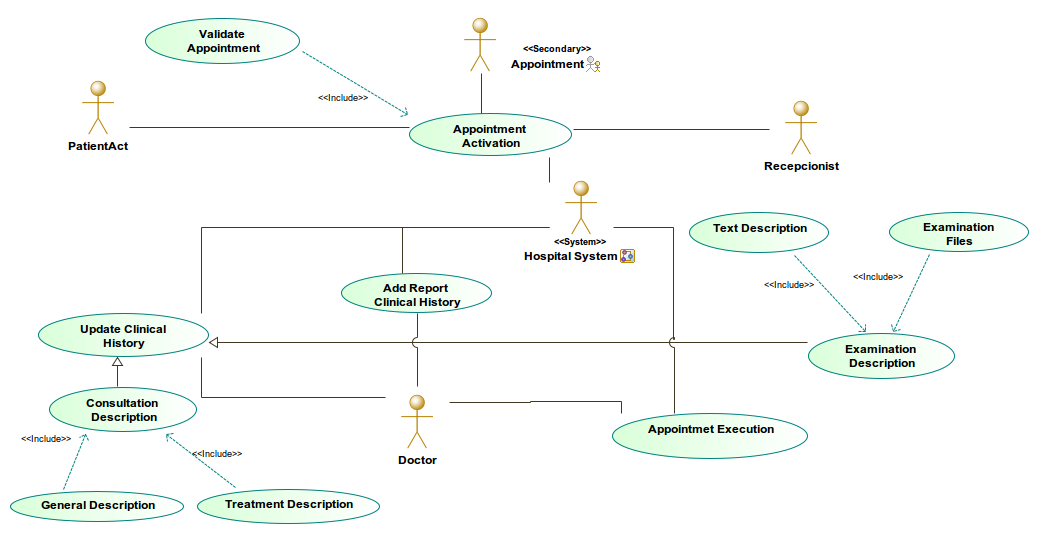
\includegraphics[width=1\linewidth]{./img/cHistories.png}
                \setcaptioncitation{Created with Modelio 3.7.}
                \caption{Examination Use Case.}
                \label{fig:examination}
            \end{figure}
            
            \subsection{Payments Use Case}

            In the payments Use Case, the appointment becomes a secondary actor by itself because the appointment is the connecting factor (somehow the product consume by the patient) between the Patient and the
            Hospital. In the diagram included in the Figure  \ref{fig:payment}, the Economy staff Actor from the hospital is introduced to review the payment status of the appointments and create penalty fees whenever is needed.
            The Economy staff uses the Hospital system to access to the appointments an patient payments.

            \begin{figure}[H]
                \centering 
                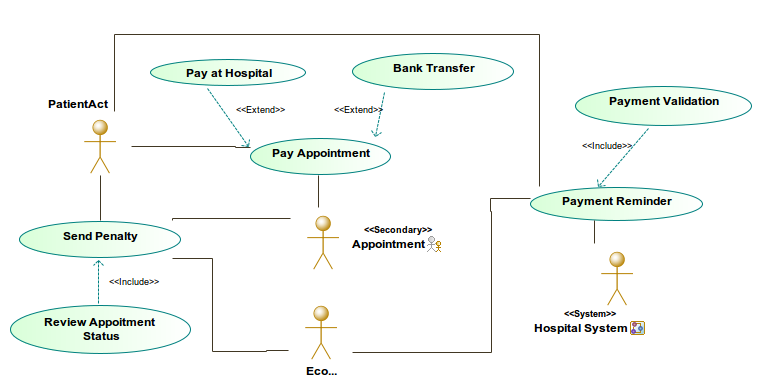
\includegraphics[width=1\linewidth]{./img/payments.png}
                \setcaptioncitation{Created with Modelio 3.7.}
                \caption{Payment Use Case Diagram}
                \label{fig:payment}
            \end{figure}

            The Patient have the option of paying at the hospital or by a bank transfer.
            
            \section{Class Diagram} 
            The Class diagram describes the attributes and operations of a class and also the constraints 
            imposed on the system. The class diagrams are widely used in the modeling of object oriented 
            systems because they are the only UML diagrams, which can be mapped directly with object-oriented languages.
            
            The class diagram explains in detail the entities with it respective attributes and operations available. It also describes the relation, multiplicity and
            association between the the different elements. The class diagram is one of the main elements when the system is design and the one that keep updating during the 
            design of the other diagrams.


            \begin{figure}[H]
                \centering 
                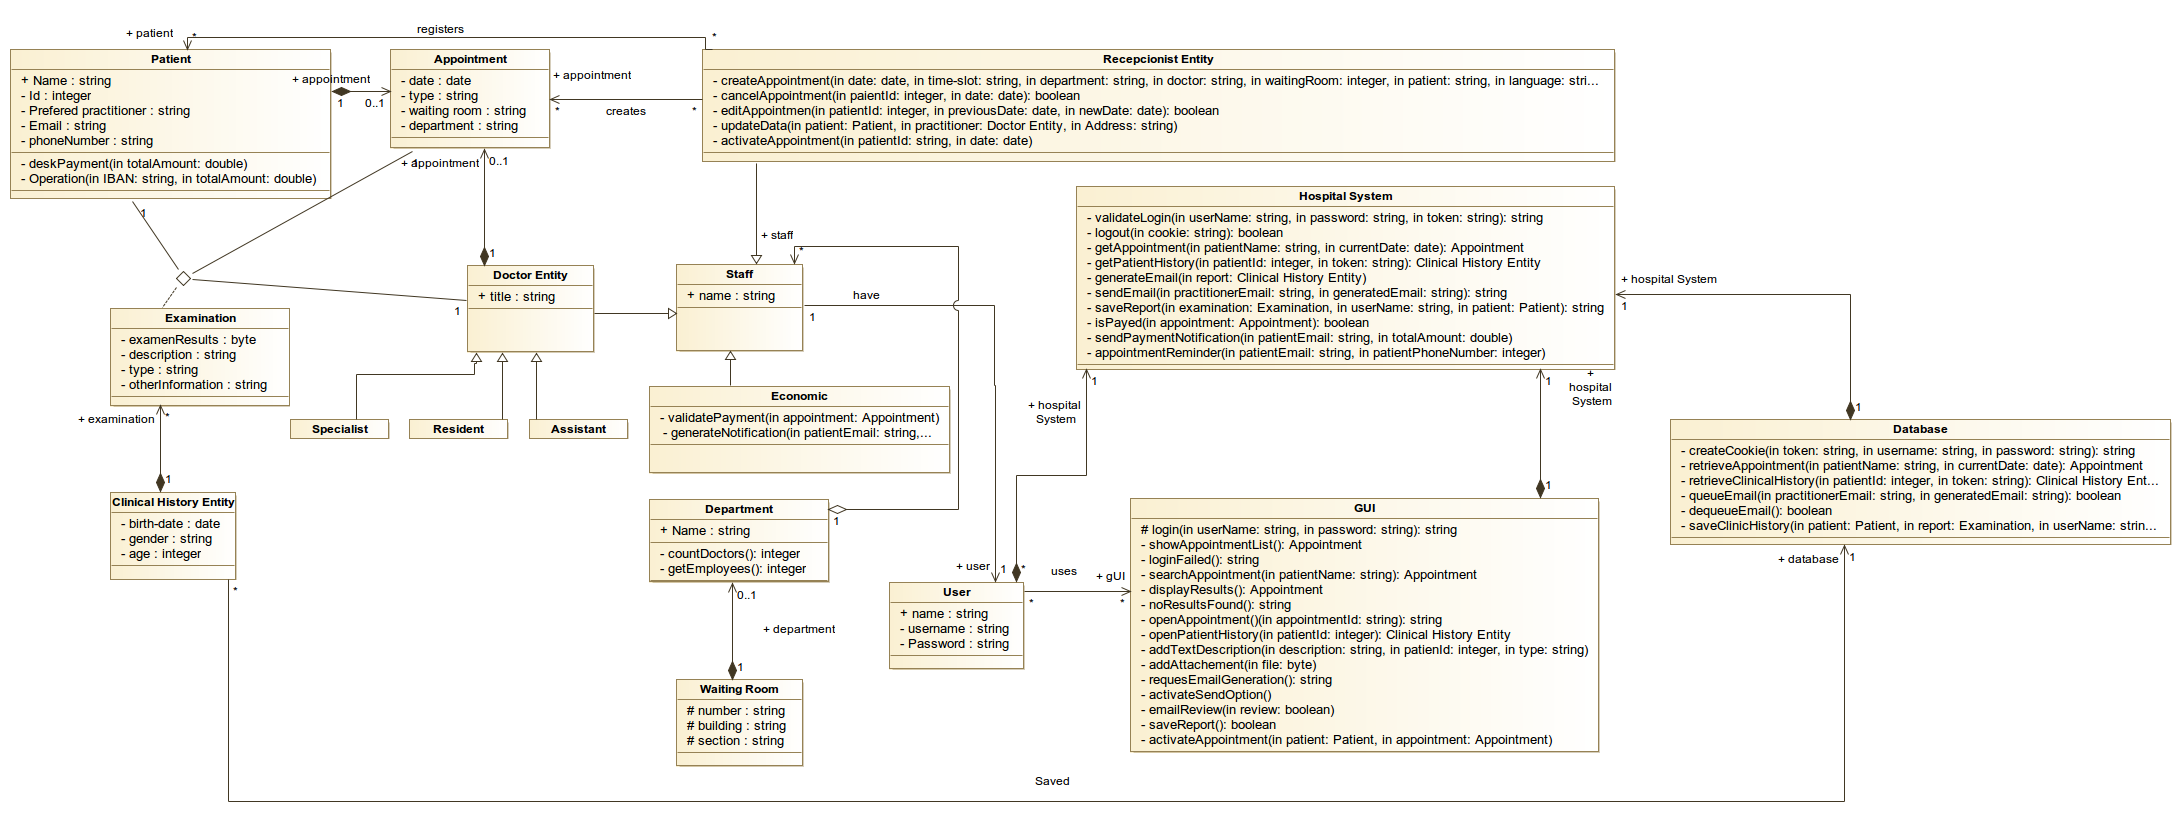
\includegraphics[width=1\linewidth]{./img/class.png}
                \setcaptioncitation{Created with Modelio 3.7.}
                \caption{Class Diagram.}
                \label{fig:class}
            \end{figure}

            In the figure \ref{fig:class} the class diagram for the hospital application is presented. All the Actors in the use case diagram became entities and some sub-classes are derive from a main class.
            A good example is the Staff class that includes all the personal working at the Hospital in different departments. At the first level is divided in Receptionist, Doctor Entity and Economic entity, and at the same time,
            the Doctor entity is generalize into Specialist, Resident and Assistance. The practitioner is considered as any of the Doctor entities that is assign to a patient.

            Additionally, the staff is associated to a Department and every Department contain waiting rooms that are addressed by a number, building and Section.

            As it was mentioned before, the hospital system is considered as a local software that manages the appointments and the clinic histories of the patients. In oder to access to the sytem, every member of the staff have an account with
            it respective user name and password. Inside the system the user interacts with a Graphical User Interface that displays the appointments, allow the receptionist to validate and schedule the appointments and the doctors to read and write the
            medical history of the patient. 

            The system also generates and schedule notifications. I like to imaging the system as a server running all the logic of the application, connected to a Database where all the Clinical Stories, Users and bills are saved.
            The GUI is part of the front-end (and middleware) of the application and the system is the back-end, using a \textit{token} to authenticate and establish the connection with the database.
            
            It is easy to identify the system controller (application) as the entity with the biggest amount of operations. This is due to its "gateway" nature to allow the  interaction between the entities and actors in the system.
            
            Some of the main functions are:

            \subsubsection{GUI operations}
            \begin{itemize}
                \item \textbf{Login(String username, String password):String =}  It allows the user to authenticate to the system and access to the Patient, appointment and billing information. This method returns an String with the new connection view for the user. It is declare as an
                String but it could also be a XML or HTML file for a web application. The login connects to the system and use the function \textit{validateFunction}.
                \item \textbf{loginFail():String =} is an operation that is triggered when the user credentials don match with the ones created in the system.
                \item \textbf{searchAppointment(String patientName):Appointment = } is the function use by the doctor to search the scheduled appointments by patient name. It will return the appointment(s) as an Appointment object that would be displayed in the GUI.
                \item \textbf{displayResults():Appointment = } display in the GUI the searched appointment.
                \item \textbf{openAppointment(String AppointmentId):String = }  request to the system the details of the appointment with an specific Id to later display them in a view.
                \item \textbf{addTextDescription(String decription, int patientIdm String type):String = } this operation receives the type of the appointment of the patient, and allow the doctor to write a description in the clinic history of the given patient.
                \item \textbf{addAttachement(byte file):void = } attaches to the report of the appointment  a string of bytes that could include images, PDF files or any other kind of document.
                \item \textbf{requestEmailGeneration():String = } request to the system to queue and email with the report fir the general practitioner of the patient. This operation does not include the patient data because I assume the system already have loaded the patient data during the appointment execution.
                It returns the ready or fail generation message.
                \item \textbf{activateSendOption():void = } prior to the email generation, the doctor has to activate and allow the send option during the report.
                \item \textbf{emailReview(Boolean review):void = } once the email is generated in the preview version of it is loaded, the Doctor had the to approve and definitively send the queued mail.
                \item \textbf{saveReport():Boolean = } save the current state of the appointment report in the clinical history. Returns true when it is successfully saved or false when there is any inconsistency.
                \item \textbf{activateAppointment(Patient patient, Appointment appointment) = } this function is used in the GUI to start the appointment and let know to the billing department that the patient attended to the schedule appointment.
            \end{itemize}
            
            \subsubsection{Hospital System operations}
            \begin{itemize}
                \item \textbf{validateFunction(String username, String password, String token):String =} This function receives the username and the password from the GUI and adds the unique token to access and validate the user in the database. This method will return a string with the view and the
                user cookie. The cookie is assigned by the database with the function \textit{createCookie}.
                \item \textbf{logout(String cookie):boolean = } destroy the cookie created for the user access. 
                \item \textbf{getAppointment(int patientId, Date currentDate):Appointment = } receives form the GUI the patientId and adds the current date to search for the available appointments of the given patient in the present day. 
                \item \textbf{getPatientHistory(int patientId, String token):Clinical History Entity = } receives from the GUI the patientId and adds the access token to retrieve the patient clinical history to the doctor.
                \item \textbf{generateEmail(Clinical History Entity report):void = } consolidates all the information of the appointment and queue an email to the patient practitioner.
                \item \textbf{sendEmail(String practitionerEmail, String generatedEmail):String = } send the report from the system to the patient practitioner.
                \item \textbf{IsPayed(Appointment appointment):boolean = } mainly used by the Economic entity to know if the patient payed the appointment bill.
                \item \textbf{sendAppointmentNotification(String patientMail, Double totalAmount):void = } send the remainder to the patient to pay the bill when is issued as a bank transfer or any other fee.
                \item \textbf{appointmentReminder(String patientEmail, int patientPhoneNumber) = } automatically sends and appointment notification by email and phone to the patient, 24 hrs before the appointment. 
                
            \end{itemize}

            \subsubsection{Database operations}
            \begin{itemize}

                \item \textbf{createCookie(String token, String username, String password): string = } the database system receives the server token together with the username and password and if the data is correct, it will return a access cookie that is saved and assigned to the user in the database.
                From this point in advance I assume and is that the cookie is included by the browser or GUI in every operation while the user remains connected and authenticated in the system.
            \end{itemize}

            Other operations used by the other entities are not described because its name explains it functionality good enough or is mentioned in other diagram.

            
            \section{Sequence Diagram}
            The sequence diagram implement is the appointment execution, involving the doctor, the hospital system and the database. The sequence diagram include some of the operations presented in the class diagram and shows entities interactions arranged in time sequence. As an important remark, I am considering that the
            Doctor is using an \textit{stateless} web application to access to the hospital system. This also explains why every action ends after the \textit{server} and \textit{database} response.

            The sequence diagram designed is vertically too long to be included in a single image. For this reason it was split in the figure \ref{fig:sequence1}, figure \ref{fig:sequence2} and figure \ref{fig:sequence3}.
           
            \begin{figure}[H]
                \centering 
                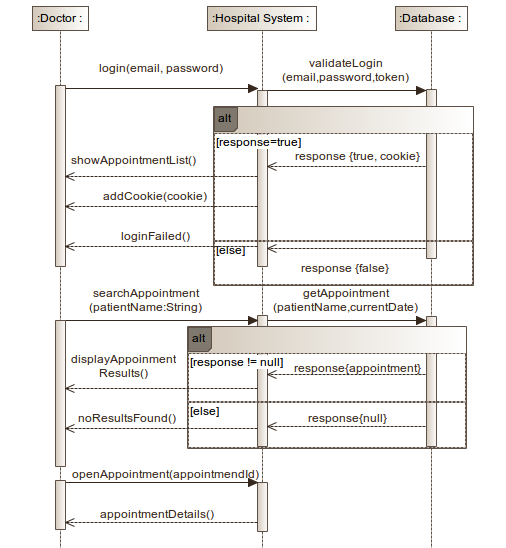
\includegraphics[width=.8\linewidth]{./img/seq1.png}
                \setcaptioncitation{Created with Modelio 3.7.}
                \caption{Sequence diagram part 1.}
                \label{fig:sequence1}
            \end{figure}

            This first part describes the Login and authentication of the Doctor as an user in the hospital system and how the Doctor search for the appointment details.
            \begin{figure}[H]
                \centering 
                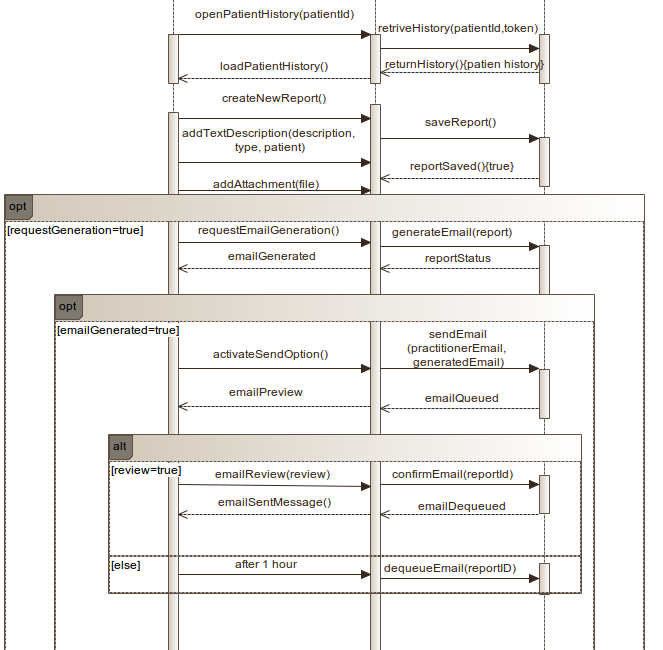
\includegraphics[width=.8\linewidth]{./img/seq2.png}
                \setcaptioncitation{Created with Modelio 3.7.e}
                \caption{Sequence diagram part 2.}
                \label{fig:sequence2}
            \end{figure}

            Continuously the Doctor creates the report by adding descriptions, files with the results or any treatment description. At the end of the report, the doctor has the option of generate, preview and send the report of the appointment to
            th patient practitioner.

            \begin{figure}[H]
                \centering 
                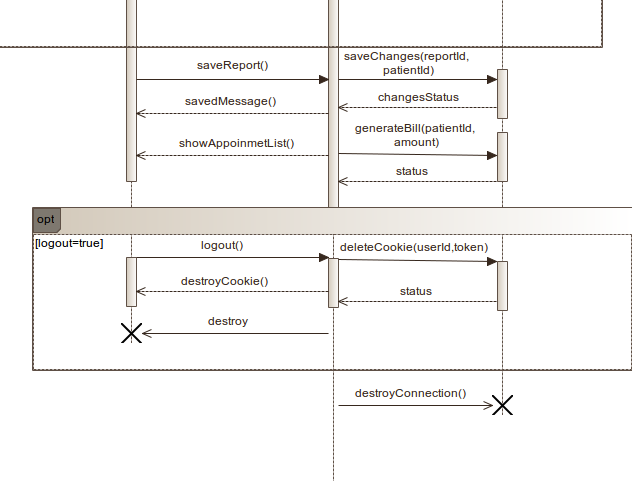
\includegraphics[width=1\linewidth]{./img/seq3.png}
                \setcaptioncitation{Created with Modelio 3.7.}
                \caption{Sequence diagram part 3.}
                \label{fig:sequence3}
            \end{figure}

            Finally in the figure \ref{fig:sequence3} illustrates hoe the report is saved in the clinical history of the patient and the creation of the bill to be paid by the patient.
            At the end of the day the Doctor is able to logout and destroy the user connection with the system.

            \section{Activity Case Diagram} 

            The activity diagrams are dynamic views of the system that expresses sequence of
            behaviors and event occurrence over time \cite{sysml}. Together
            with the state diagram, the system behavior is expressed.

            The activity diagram  somehow divides the hospital management in processes. In the figure \ref{fig:activity} the activity diagram is explained in 8 parts:

            \begin{itemize}
                    \item \textbf{Appointment Creation}
                    \item \textbf{Patient Registration}
                    \item \textbf{Assign Doctor}
                    \item \textbf{Modify Appointment}
                    \item \textbf{Cancel Appointment}
                    \item \textbf{Appointment Reminder}
                    \item \textbf{Cancel Appointment}
                    \item \textbf{Appointment Execution}
                    \item \textbf{Appointment Payment}
            \end{itemize}

            At the same time every activity contains sub-activities that are required to finish an activity before going to the next one.
            
            \begin{figure}[H]
                \centering 
                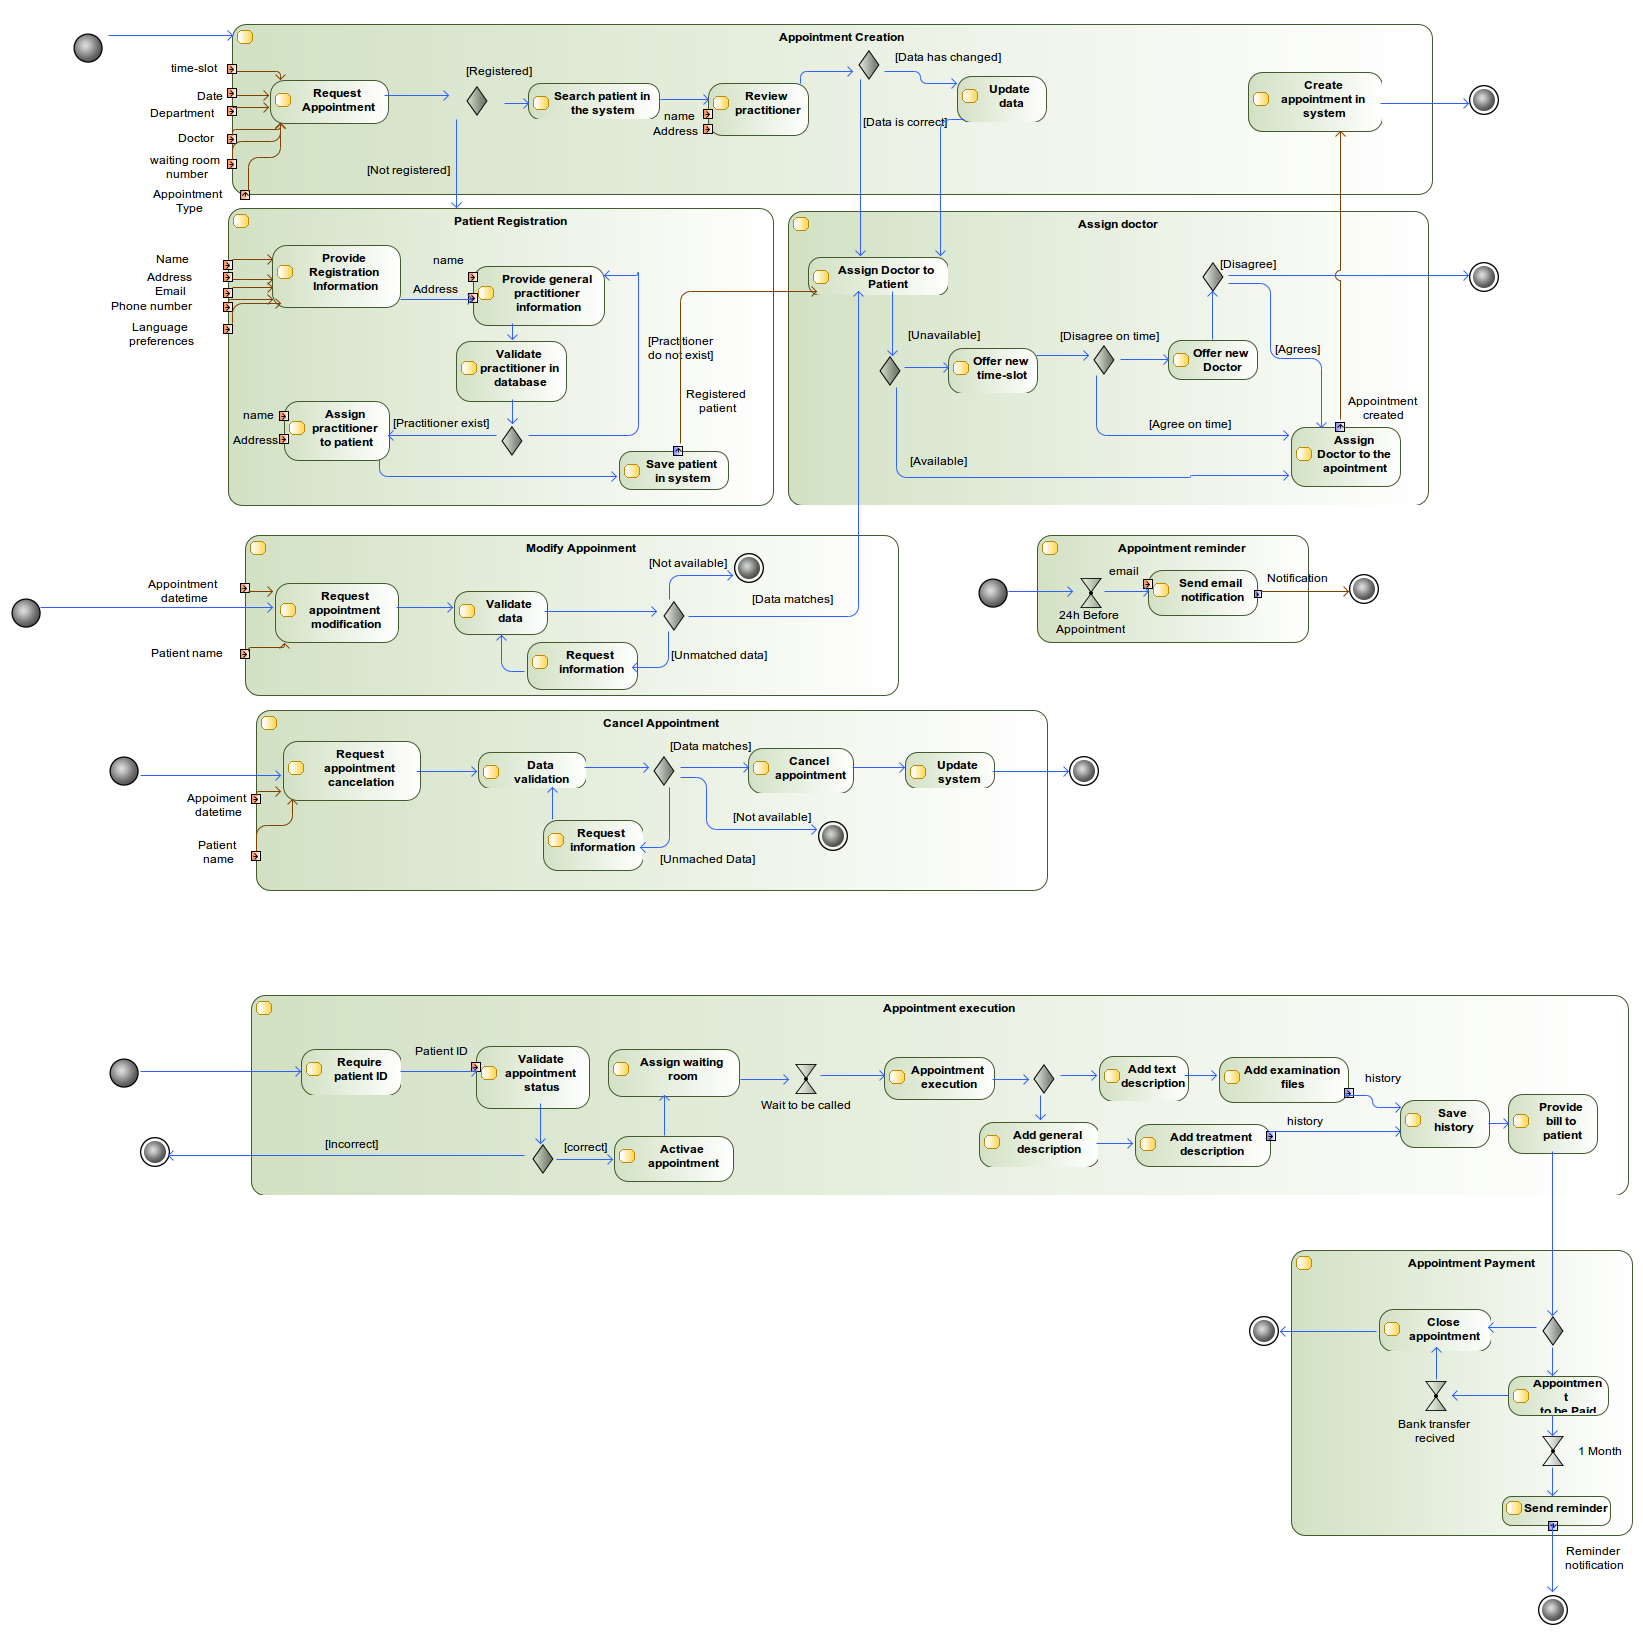
\includegraphics[width=1\linewidth]{./img/Activity.png}
                \setcaptioncitation{Created with Modelio 3.7.}
                \caption{Activity Diagram.}
                \label{fig:activity}
            \end{figure}

            The activity diagram designed intents to explain the entire appointment process, from the request of the appointment by the patient, until the execution and the appointment payment. This 
            diagram also consider the inputs, outputs and decision in every activity.

            \section{State Diagram}
           
            Next to the activity diagram is the State Diagram, which is also a behavior
            diagram focus on how a structure within a system changes in response to event
            occurrences over time. It refers to the behavior that begins executing the moment a block
            is instantiated and generally finishes executing when that instance is destroyed.
            
            The developed state diagram developed in the figure \ref{fig:state} represents all the possible states for the appointment entity and all the responsible actions that makes the appointment to exit or entry into a 
            determined state.

            \begin{figure}[H]
                \centering 
                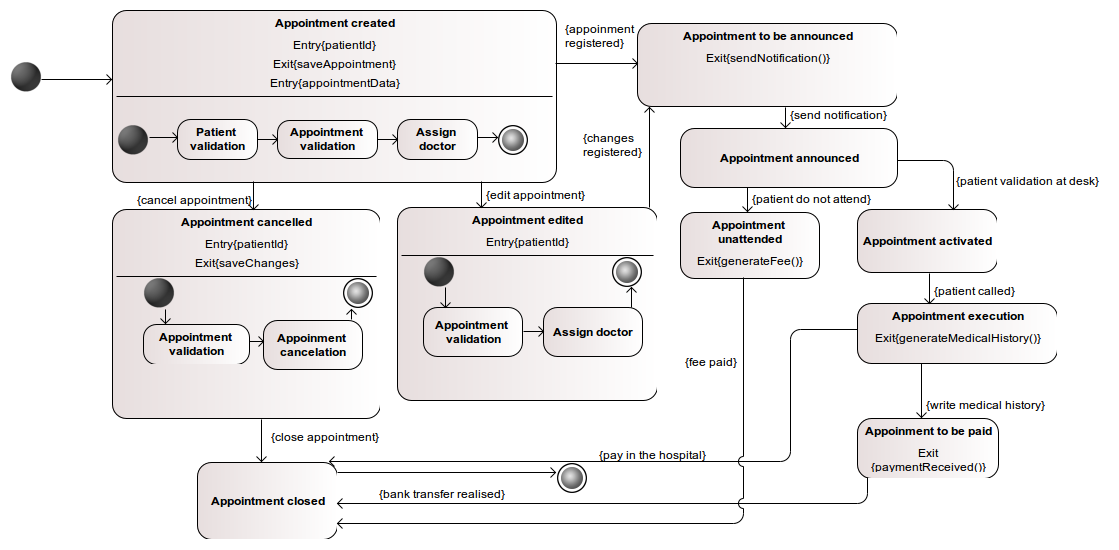
\includegraphics[width=.8\linewidth]{./img/state.png}
                \setcaptioncitation{Created with Modelio 3.7.}
                \caption{State Diagram}
                \label{fig:state}
            \end{figure}
            
            There are 10 possible states, 7 sub-states and more than 12 operations for the appointment. All the operations are also included in the class diagram and  better explained with the respective arguments and return values.
            
        
            \newpage
            \bibliography{report}
            \bibliographystyle{ieeetr}
            \nocite{*}
    \end{document}